\documentclass[a0]{tumposter}

\usepackage[english]{babel}

\usepackage{blindtext}

\usepackage{multicol}
\usepackage{amsmath}
\usepackage{graphicx}

% for printing fontsizes
\usepackage{printlen}
\uselengthunit{mm}



\usepackage{microtype}
\usepackage{graphicx}
%\usepackage{subfigure}
\usepackage{booktabs} 
\usepackage{hyperref}
\newcommand{\theHalgorithm}{\arabic{algorithm}}
%\usepackage[accepted]{icml2019}


\setlength{\abovecaptionskip}{5pt plus 3pt minus 2pt}
%\setcitestyle{numbers,round,citesep={;},aysep={,},yysep={;}}

\usepackage{times}
\usepackage{epsfig}
\usepackage{graphicx}
\usepackage{amsmath}
\usepackage{amssymb}
\usepackage[utf8]{inputenc}
%\usepackage{booktabs}
\setlength{\tabcolsep}{5pt}
%\usepackage{subcaption}
\usepackage{tumabbrev}

\usetikzlibrary{backgrounds}

\usepackage{appendix}

% Include other packages here, before hyperref.

% If you comment hyperref and then uncomment it, you should delete
% egpaper.aux before re-running latex.  (Or just hit 'q' on the first latex
% run, let it finish, and you should be clear).
%\usepackage[breaklinks=true,bookmarks=false]{hyperref}


\usepackage[capitalize]{cleveref}
%\usepackage[square,sort,comma,numbers]{natbib}
%\usepackage{natbib}

%% this hack seems to be nececessary due to incompatibilities of cvpr template and tikz... -> https://tex.stackexchange.com/questions/398223/tikz-gives-error-command-everyshipouthook-already-defined
%\makeatletter
%\@namedef{ver@everyshi.sty}{}
%\makeatother
%% hackend

\usepackage{tikz}
\usepackage{pgfplots}
\usetikzlibrary{positioning, calc,arrows,arrows.meta, fit}
%\usetikzlibrary{arrows.meta,calc,decorations.markings,math,arrows.meta}
\usepgfplotslibrary{groupplots}
\usepgfplotslibrary{fillbetween}
\usepgfplotslibrary{statistics} % provides boxplots
\usepackage{xfrac}

\usetikzlibrary{shapes,snakes}

\newcommand{\tp}{tp}
\newcommand{\tn}{tn}
\newcommand{\fp}{fp}
\newcommand{\fn}{fn}


\usepackage{tumcolors}
\usepackage{tummath}
\newcommand{\yhat}{\hat{\V{y}}}
\newcommand{\ycorrect}{\hat{y}^+}
\newcommand{\thetadelta}{\V{\Theta}_\delta}
\newcommand{\biasdelta}{b_\delta}
\newcommand{\biasclass}{\V{b}_\text{c}}
\newcommand{\thetaclass}{\V{\Theta}_\text{c}}
\newcommand{\thetafeat}{\V{\Theta}_\text{feat}}
\newcommand{\fclass}{f_\text{c}}
\newcommand{\fdelta}{f_\delta}
\newcommand{\ffeat}{f_\text{feat}}
\newcommand{\f}{f}

\newcommand{\rvtime}{T_c} 
\newcommand{\xuptot}{\M{X}_{\rightarrow t}} 
\newcommand{\deltauptot}{\delta_{\rightarrow t}} 
\newcommand{\tstop}{\ensuremath{t_\text{stop}}}
\newcommand{\meantstop}{\ensuremath{\bar{t}_\text{stop}}}
\usepackage[super]{nth}
\usepackage{mathtools}

\definecolor{evalcolor}{HTML}{3F3F3F}
\definecolor{traincolor}{HTML}{B98951}
\definecolor{validcolor}{HTML}{3F4BBE}

\colorlet{colortrain}{tumdiagramred}
\colorlet{colorinfer}{tumblack}

\colorlet{earlinesscolor}{tumblue}
\colorlet{accuracycolor}{tumorange}

\colorlet{stdcolor}{tumbluelight}
\colorlet{mediancolor}{tumorange}
\colorlet{meancolor}{tumblue}

\colorlet{ecolor}{tumorange}
\colorlet{ccolor}{tumblue}


\colorlet{colorclassone}{tumblue}
\colorlet{colorclasstwo}{tumblack}
\colorlet{colorclassthree}{tumgreen}
\colorlet{colorclassfour}{tumorange}
\colorlet{colorblue}{tumblue}

%\colorlet{b1color}{tumdiagramaubergine}
%\colorlet{b2color}{tumdiagramnavyblue}
%\colorlet{b3color}{tumdiagramturquoise}
%\colorlet{b4color}{tumdiagramgreen}
%\colorlet{b5color}{tumdiagramlimegreen}
%\colorlet{b6color}{tumdiagramyellow}
%\colorlet{b7color}{tumdiagramsand}
%\colorlet{b8color}{tumdiagramredorange}
%\colorlet{b8Acolor}{tumdiagramred}
%\colorlet{b9color}{tumblack}
%\colorlet{b10color}{tumblue}
%\colorlet{b11color}{tumdiagramdarkred}
%\colorlet{b12color}{tumorange}

% atmospheric bands
\colorlet{b1color}{tumblack}%tumdiagramaubergine
\colorlet{b9color}{tumblack}%tumblack
\colorlet{b10color}{tumblack}%tumblue

%visisble bands
\colorlet{b2color}{tumblue}%tumdiagramnavyblue
\colorlet{b3color}{tumblue}%tumdiagramturquoise
\colorlet{b4color}{tumblue}%tumdiagramgreen

% near infrared bands
\colorlet{b5color}{tumdiagramred}%tumdiagramlimegreen
\colorlet{b6color}{tumdiagramred}%tumdiagramyellow
\colorlet{b7color}{tumdiagramred}%tumdiagramsand
\colorlet{b8color}{tumdiagramred}%tumdiagramredorange
\colorlet{b8Acolor}{tumdiagramred}%tumdiagramred

% SWIR bands
\colorlet{b11color}{tumorange}%tumdiagramdarkred
\colorlet{b12color}{tumorange}%tumorange

\colorlet{epsilon0color}{tumorange}
\colorlet{epsilon1color}{tumblue}
\colorlet{epsilon10color}{tumblack}

\colorlet{meadowcolor}{tumbluemedium}
\colorlet{wbarleycolor}{tumbluedark}
\colorlet{corncolor}{tumorange}
\colorlet{wheatcolor}{tumgreen}
\colorlet{sbarleycolor}{tumdiagramred}
\colorlet{clovercolor}{tumdiagramturquoise}
\colorlet{triticalecolor}{tumdiagramsand}

\tikzstyle{rnn}=[draw,circle, inner sep=.1em]
\tikzstyle{norm}=[rounded corners,draw]
\tikzstyle{annot}=[rounded corners, fill=tumblue!20]
\tikzstyle{infer}=[-{stealth[scale=10]}, shorten >=.0em, shorten <=.0em, colorinfer, thick]
\tikzstyle{loss}=[fill=tumblue!10, rounded corners, font=\small, thick]
\tikzstyle{grad}=[colortrain, thick]

\newcommand{\ptoffset}{\varepsilon}

\tikzstyle{test} = [thick]
\tikzstyle{train} = [thin, dotted]

\usepackage[inline]{enumitem}
\setenumerate{label=(\roman*),itemsep=3pt,topsep=3pt}

 \setlength{\belowcaptionskip}{-10pt}
%\usepackage{titlesec}
%\titlespacing{\section}{0pt}{10pt}{3pt}


\newcommand{\deltat}{\ensuremath{p_t}}

\usetikzlibrary{external}
\tikzexternalize[prefix=tikz/]
%\tikzexternalize
\tikzexternaldisable

\usepackage[eulergreek]{sansmath}
\pgfplotsset{
	y tick label style={/pgf/number format/.cd,%
		scaled y ticks = false,
		set thousands separator={},
		fixed},
	x tick label style={/pgf/number format/.cd,%
		scaled x ticks = false,
		set decimal separator={,},
		fixed},
	tick label style = {font=\scriptsize\sansmath\sffamily},
	every axis label = {
		font=\scriptsize\sansmath\sffamily},
	every axis/.append style={
		axis lines=left, 
		enlargelimits, 
		thick},
	legend style = {font=\scriptsize\sansmath\sffamily, draw=none, rounded corners, fill opacity=.5, text opacity=1},
	label style = {font=\scriptsize\sansmath\sffamily},
	grid style={line width=.1pt, draw=gray!10},
	major grid style={line width=.2pt,draw=tumgraylight},
}

\let\tempone\itemize
\let\temptwo\enditemize
\renewenvironment{itemize}{\tempone\addtolength{\itemsep}{-.5\baselineskip}}{\temptwo}


\tikzstyle{circ} = [circle, draw=white, fill=tumblue, inner sep=.08em]
\newcommand{\fcn}{
	\begin{tikzpicture}[scale=.5, rotate=0, baseline=-.25em, inner sep=1pt]
	\node[circ](a0) at (0,-1){};
	\node[circ](a1) at (0,0){};
	\node[circ](a2) at (0,1){};
	
	\node[circ](b0) at (1,-0.5){};
	\node[circ](b1) at (1,0.5){};
	
	\draw[-] (a0) -- (b0);
	\draw[-] (a1) -- (b0);
	\draw[-] (a2) -- (b0);
	
	\draw[-] (a0) -- (b1);
	\draw[-] (a1) -- (b1);
	\draw[-] (a2) -- (b1);
	
	\end{tikzpicture}
}

\newcommand{\hidden}[1]{
	\begin{tikzpicture}[scale=.1, baseline=-.25em]	
	%\draw[step=1.0,black,thin] (0,0) grid (#1,1);
	\foreach \i in {1,...,#1}{
		\node[circle, draw=white, fill=tumbluelight, inner sep=1pt] at (\i,0){};
	}
	\end{tikzpicture}
}

\newcommand{\drawvector}[1]{
	\begin{tikzpicture}[scale=.1, baseline=-.25em]	
	%\draw[step=1.0,black,thin] (0,0) grid (#1,1);
	\foreach \i in {1,...,#1}{
		\node[circ] at (\i,0){};
	}
	\end{tikzpicture}
}

\tikzstyle{druschdatum} = [thin, star,star points=3, star point ratio=0.5, inner sep=.15em, draw=tumwhite, fill=tumblue]

\newcommand{\druschdatum}{
\begin{tikzpicture}[scale=2, baseline=-.25em, inner sep=0]
\node[druschdatum, inner sep=.25em]{};
\end{tikzpicture}
}

\usepackage[utf8]{inputenc}

\title{
	Early Classification for Agricultural Monitoring \\ from Satellite Time Series
	}
	
\author{
	Marc Rußwurm,\footnotemark[1] Romain Tavenard,\footnotemark[2] Sébastien Lefèvre,\footnotemark[2] Marco Körner\footnotemark[1]
	}

\header{
	Remote Sensing Technology \\
	TUM Department of Civil, Geo and Environmental Engineering \\
	Technical University of Munich
	}
	
\begin{document}
\maketitle

\renewcommand{\subsection}[1]{\textbf{#1}}

\begin{minipage}[t]{.65\textwidth}
	
	\section{Objective}
	
	
	\begin{tikzpicture}[scale=16.8]
	\node[label={[name=sat,text height=1.5ex,text depth=.25ex]Satellite Data}, anchor=north](x) at (-1,0){$\M{X} = (\V{x}_0, \V{x}_1, \dots , \V{x}_T)$};
	\node[below=of x, label={[yshift=1.3em, xshift=1.8em, font=\tiny, text=white]below:ESA Sentinel 2 Satellite}](s2){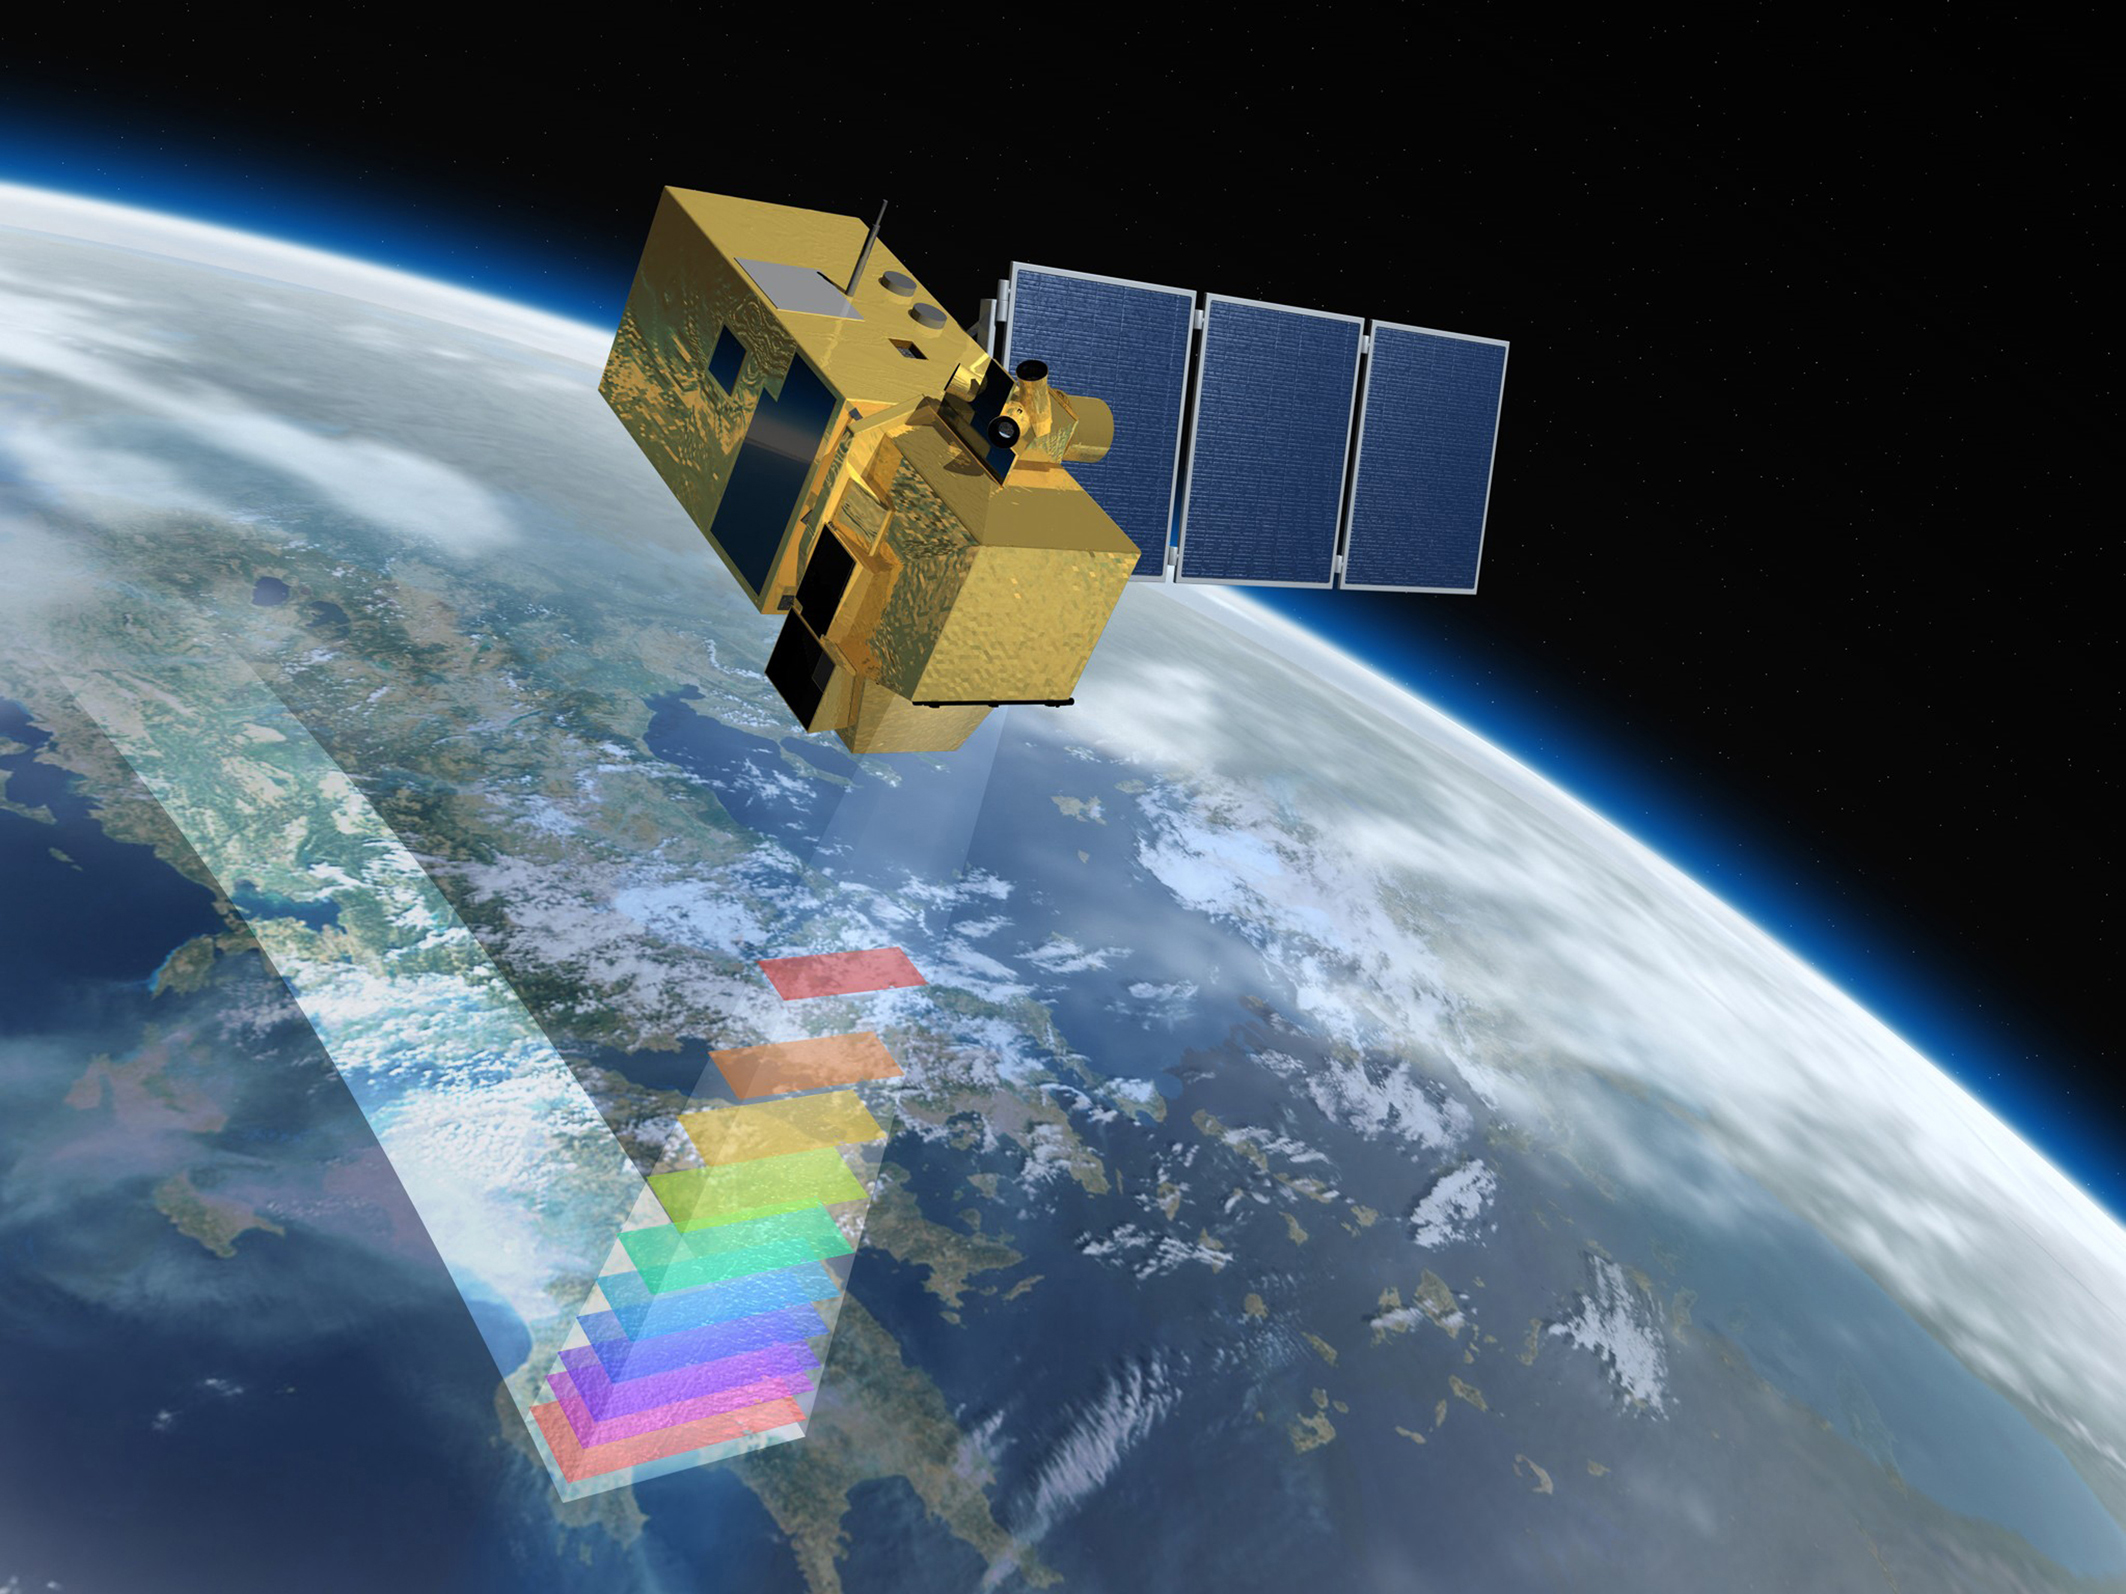
\includegraphics[width=11cm]{images/sentinel2}};
	
	
	\node[below=0em of s2, text width=11cm](eqbox){
		\small
		\begin{itemize}
			\item collected at regular temporal intervals of 2-3 days
			\item measurements of 13 spectral bands
			\item data available globalls
		\end{itemize} 
	};
	
	\node[label={[name=cm,text height=1.5ex,text depth=.25ex]{Early} {Classification} Model}, anchor=north](f) at (0,0){ $\yhat_t, {\deltat} = f(\xuptot)$};
	\node[below=0em of f, text width=13cm, font=\small](info){
		\begin{description}
		
		\item[$\xuptot$] observation until $t$  \\
		\item[$\yhat_t$] class prediction scores \\
		\item[$\deltat$] probability of stopping.
		
		\end{description}
		
	};
%	\node[below=of f](example){\tikzsetnextfilename{example}
\begin{tikzpicture}[rounded corners=0pt]
	
	\tikzstyle{annot} = [font=\verytiny\sffamily, text=tumblue]
	\tikzstyle{point} = [very thin, tumbluelight, shorten >= .25em, shorten <= .25em]
	
	% from /home/marc/projects/EV2019/images/example/tstop.txt
	\def\tstopv{0.6285714285714286}
	\def\class{winter barley}
	
	\begin{groupplot}[
	group style={
		group name=my plots,
		group size=1 by 2,
		columns=1,
		xlabels at=edge bottom,
		xticklabels at=edge bottom,
		vertical sep=1em,
	},
	ylabel near ticks,
	ylabel style={font=\sffamily\small, rotate=-90},
	width=.9\textwidth,
	height=5cm,
	axis x line=bottom,
	axis y line=left,
	enlarge x limits=0.01,
	xtick={0,0.25,0.5,0.75,1},
	xticklabels={January,April,June,Sepember,December},
	ymajorgrids,
	ymin=0, ymax=1.4
	]
	
	\nextgroupplot[very thin,
		no marks,  
		ylabel={$\M{x}$},
		draw opacity=.8,
		smooth,
		legend columns=2,
		legend style={at={(.5,1.2)},anchor=south, line width=1pt, fill=tumblue!10}
		]
		 
	\addplot[b1color] table [x=t, y=B1, col sep=comma, forget plot] {images/example/input.csv};
	\addplot[b9color] table [x=t, y=B9, col sep=comma, forget plot] {images/example/input.csv};
	\addplot[b10color] table [x=t, y=B10, col sep=comma] {images/example/input.csv};
	
	\addplot[b11color] table [x=t, y=B11, col sep=comma, forget plot] {images/example/input.csv};
	\addplot[b12color] table [x=t, y=B12, col sep=comma] {images/example/input.csv};
	
	\addplot[b5color] table [x=t, y=B5, col sep=comma, forget plot] {images/example/input.csv};
	\addplot[b6color] table [x=t, y=B6, col sep=comma, forget plot] {images/example/input.csv};
	\addplot[b7color] table [x=t, y=B7, col sep=comma, forget plot] {images/example/input.csv};
	\addplot[b8color] table [x=t, y=B8, col sep=comma, forget plot] {images/example/input.csv};
	\addplot[b8Acolor] table [x=t, y=B8A, col sep=comma] {images/example/input.csv};
		
	\addplot[b2color] table [x=t, y=B2, col sep=comma, forget plot] {images/example/input.csv};
	\addplot[b3color] table [x=t, y=B3, col sep=comma, forget plot] {images/example/input.csv};
	\addplot[b4color] table [x=t, y=B4, col sep=comma] {images/example/input.csv};
	
	
	\draw[fill=white, draw=none, opacity=.5] (axis cs:\tstopv,0) rectangle (axis cs:1,1.1);
	
	\node[annot](cllab) at (axis cs:.2,1.3) {clouds (noise)};
	\draw[point] (cllab) -- (axis cs:.13,.7);
	\draw[point] (cllab) -- (axis cs:.25,.7);
	\draw[point] (cllab) -- (axis cs:.53,1);
	\draw[point] (cllab) -- (axis cs:.45,.85);
	
	\node[annot](glab) at (axis cs:.9,1.3) {ground (signal)};
	\draw[point] (glab) -- (axis cs:.38,.3);
	\draw[point] (glab) -- (axis cs:.21,.3);
	\draw[point] (glab) -- (axis cs:.7,.3);
	
	\draw (axis cs:\tstopv,0) -- (axis cs:\tstopv,1) node[above, font=\tiny]{$\tstop(\deltat)$};
	
	
	
	\legend{3 atmospheric bands, 2 short-wave infrared bands, 5 near infrared bands, 3 visible bands (RGB)}
	
	
	\nextgroupplot[very thin,
		smooth,
		no marks, 
		ylabel={$\yhat$},
		legend style={at={(.5,-.5)},anchor=north, line width=1pt, fill=tumblue!10, font=\scriptsize},
		legend columns=4]	
	
	\addplot[meadowcolor] table [x=t, y=meadows, col sep=comma] {images/example/proba.csv};
	\addplot[wbarleycolor, thick] table [x=t, y=winter barley, col sep=comma] {images/example/proba.csv};
	\addplot[corncolor] table [x=t, y=corn, col sep=comma] {images/example/proba.csv};
	\addplot[wheatcolor,] table [x=t, y=winter wheat, col sep=comma] {images/example/proba.csv};
	\addplot[sbarleycolor] table [x=t, y=summer barley, col sep=comma] {images/example/proba.csv};
	\addplot[clovercolor] table [x=t, y=clover, col sep=comma] {images/example/proba.csv};
	\addplot[triticalecolor] table [x=t, y=winter triticale, col sep=comma] {images/example/proba.csv};
	
	\draw[fill=white, draw=none, opacity=.5] (axis cs:\tstopv,0) rectangle (axis cs:1,1);
	
	\draw (axis cs:\tstopv,0) -- (axis cs:\tstopv,2.2);
	
	\node[annot](rand) at (axis cs:.1,.8) {first hints};
	\draw[point] (rand) -- (axis cs:.2,.15);
	
	\node[annot](wrong) at (axis cs:.17,1.1) {initially wrong predictions};
	\draw[point] (wrong) -- (axis cs:.25,.7);
	\draw[point] (wrong) -- (axis cs:.4,1);
	
	\node[annot, align=center](corrwait) at (axis cs:.4,1.3) {waiting for more data};
	\draw[point] (corrwait) -- (axis cs:.5,.8);
	
	\node[annot](corr) at (axis cs:.8,1.3) {seen enough data};
	\draw[point] (corr) -- (axis cs:.63,1);
	
	\legend{meadows,\textbf{winter barley},corn,winter wheat,summer barley,clover,winter triticale}
	
	
%	\addplot[thick,colorclassone, name path=y1] table[x=t, y=y1]{\mydata};
%	\addplot[thick,colorclasstwo, name path=y2] table[x=t, y=y2]{\mydata};
%	\addplot[thick,colorclassthree, name path=y3] table[x=t, y=y3]{\mydata};
%	\addplot[thick,colorclassfour, name path=y4] table[x=t, y=y4]{\mydata};
	%\addplot[colorblue!20] fill between[of = y1 and axis];
	%\addplot[colorhgray!20] fill between[of = y2 and axis];
	%\addplot[colorgreen!20] fill between[of = y3 and axis];
	%\addplot[colororange!20] fill between[of = y4 and axis];
	
	
	\end{groupplot}
	
%	\node[font=\sffamily\tiny, anchor=west] at (-.4,3.3) {All 13 spectral bands of the Sentinel 2 satellites grouped by spectral signature};
%	\node[font=\sffamily\tiny, anchor=west] at (0,-3.1) {predicted crop type classes (correct class in \textbf{bold})};
%	
	\end{tikzpicture}};
	\node[circle, below=of info, text width=11cm, fill=tumbluedark, text=white](example){Classifying a \\ satellite time series \\ {\color{tumbluelight}\textbf{accurately}} \color{white} as {\color{ecolor}\textbf{early}} \color{white} as possible};
	
	
	\node[label={[name=ctm,text height=1.5ex,text depth=.25ex]Crop Type Labels}, anchor=north](y) at (1,0){
		$\V{y} = \small (y_\text{corn}, y_\text{barley}, \dots) \in \mathbb{R}^{13}$
	};
	\node[below=of y, label=below:crop type labels](labels){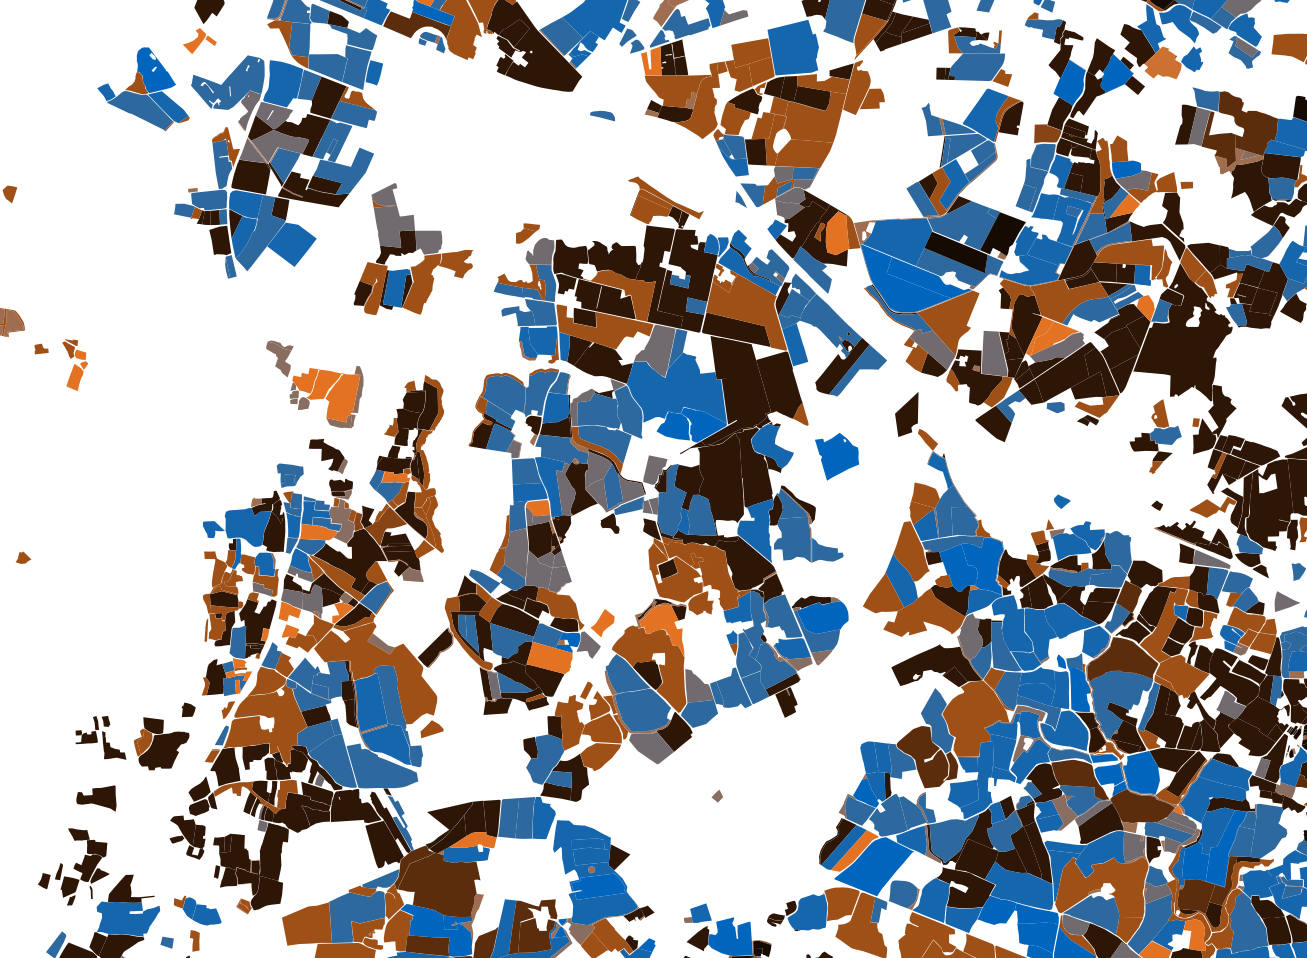
\includegraphics[width=11cm]{images/parcels}};
	\node[below=of labels, text width=11cm](lbls){
		\small
		\begin{itemize}\setlength\itemsep{.1em}
		\item European Common Agricultural Policy (CAP)
		\item collected yearly in entire Europe
%		\item slowly made publicly available
%		\item today, gathered on a national basis
%		\item in future harmonized within Europe's INSPIRE directive
		\end{itemize}
	};
	
	\draw[very thick, -{Stealth[scale=.5]}, tumblue] (x) -- (f);
	\draw[very thick, -{Stealth[scale=.5]}, tumblue] (f) -- (y);
	
	\coordinate(bottomleftcolumn) at (example.south -| s2);
	\coordinate(bottomrightcolumn) at (example.south -| lbls);
	
	\scoped[on background layer]
	{
		\node[fit=(ctm)(lbls)(bottomrightcolumn), fill=tumbluelight!20, inner sep=1em, rounded corners]{};
		\node[fit=(f)(example)(cm), fill=tumorange!20, inner sep=1em, rounded corners]{};
		\node[fit=(sat)(eqbox)(bottomleftcolumn), fill=tumbluelight!20, inner sep=1em, rounded corners]{};
	}	
	
	\end{tikzpicture}
	
	
	\section{Method}
	
	Based on previous work (Rußwurm et al., 2019) applied to crop type mapping from remote sensing data.
	
	%A network output to indicate a probability of stopping $\deltat$
	
	\begin{minipage}[t]{.49\textwidth}
		\subsection{Mechanism}
		
		\newcommand{\backpropstoppingrulefull}{
\tikzsetnextfilename{backprop_stopping_rule}

\begin{tikzpicture}[node distance=1em and 1em]
\node[](x0){$\V{x}_t$};
\node[rnn, below=of x0](h0){$\V{h}_t$};  %$\theta_\text{rnn}$};
\node[below right= 2em and 1em of h0](y0){$\yhat_t$};
\node[left=1.1em of x0,text=tumgraydark](xprev){$\V{x}_{t-1}$};
\node[right=1.5em of x0,text=tumgraydark](xnext){$\V{x}_{t}$};
\node[rnn, left=1.5em of h0,draw=tumgray](hprev){\phantom{$h_t$}};
\node[rnn, right=1.5em of h0,draw=tumgray](hnext){\phantom{$h_t$}};
\node[below left= 2em and 1em of h0](d0){$\deltat$};

\node[loss, below=of y0](L0){$\mathcal{L}_c$}; % -1em
%\node[right=of L0](t0){$\V{y}_t$};
\draw[-stealth, grad] (y0) -- (L0);
%\draw[-stealth, grad] (t0) -- (L0);

\draw[infer, draw=tumgray] (xprev) -- (hprev);
\draw[infer, draw=tumgray] (xnext) -- (hnext);

\draw[infer] (x0) -- (h0);
\draw[infer,draw=tumgray] (hprev) -- (h0);
\draw[infer,draw=tumgray] (h0) -- (hnext);
\draw[infer] (h0) -- (y0) node[midway,right, text=black](wc){$\theta_{cl}$};
\draw[infer] (h0) -- (d0) node[midway,left, text=black](wd){$\theta_{p}$};

\draw[-stealth, grad] (L0) to [bend right=30] node[near end, right, text=colortrain]{$\frac{\partial\mathcal{L}}{\partial\theta_\text{cl}}$}
(wc);

\node[below=of d0](pt){$P(t)$};
\node[below=8em of h0, loss](L){$\mathcal{L}_t$}; % = P(t)\mathcal{L}_c (\xuptot, y)$}; (\xuptot, y ; \alpha)

%\node[left=.5em of pt](budget){$P(t;\deltauptot)$};

\draw[infer] (L0) -- (L);
\draw[infer] (d0) -- (pt);
\draw[infer] (pt) -- (L);
%\draw[infer] (budget) -- (pt);

\draw[-stealth, grad] (L) to [bend right=30] node[midway, right, text=colortrain]{$\frac{\partial\mathcal{L}}{\partial\mathcal{L}_c}$}(L0);

\draw[-stealth, grad] (L) to [bend left=30] node[midway, left, text=colortrain]{$\frac{\partial\mathcal{L}}{\partial P(t)}$}(pt);

\draw[-stealth, grad] (pt) to [bend left=30] node[midway, left, text=colortrain]{$\frac{\partial\mathcal{L}}{\partial \theta_{p}}$}(wd);

%\node[left= 3em of h0]{
%
\tikzstyle{dummy} = [inner sep=0]
\tikzstyle{flow} = [thin, -{Stealth[scale=.5]}]
\tikzstyle{endflow} = [flow, shorten >= 0, shorten <= 0]
\tikzstyle{operator} = [inner sep=0, font=\scriptsize]
\tikzstyle{conn} = [-stealth, shorten >= .2em, inner sep=0]
\tikzstyle{conntime} = [conn, tumgray]
\tikzstyle{lstmcell} = [inner sep=0, fill=tumbluelight!20, rounded corners=1em]


\newcommand{\act}{
	\begin{tikzpicture}[scale=.3]
		\node[circle, draw]{
			\begin{tikzpicture}
			\draw (0,0) to[out=0, in=180] (1,1);
			\end{tikzpicture}
		}
	\end{tikzpicture}	
}



\newcommand{\lstm}{
	\begin{tikzpicture}[inner sep=0, xscale=2, yscale=2]
	\coordinate (-input) at (0,1); % top left
	\coordinate (-output) at (0,-2.75); % top left
	\node[inner sep=0](fgate) at (-1.5,0){\fcn};
	\node[inner sep=0](igate) at (-.5,0){\fcn};
	\node[inner sep=0](jgate) at (.5,0){\fcn};
	\node[operator](jmult) at (0,-1.25) {$ \odot $};
	\draw[endflow] (jgate) -- (jmult);
	\draw[endflow] (igate) -- (jmult);
	\node[inner sep=0](ogate) at (1.5,0){\fcn};

	\draw[endflow] (-input) to[out=270,in=90] (ogate.north);
	\draw[endflow] (-input) to[out=270,in=90] (jgate.north);
	\draw[endflow] (-input) to[out=270,in=90] (igate.north); 
	\draw[endflow] (-input) to[out=270,in=90] (fgate.north);

	\node[operator](fmult) at (-1,-1.25) {$ \odot $};
	\draw[endflow] (fgate) -- (fmult); 
	\node[operator](cadd) at (0,-1.75) {$\oplus$};
	\draw[endflow] (jmult) -- (cadd); 
	\draw[endflow] (fmult) -- (cadd);		
	
	\node[operator](outtanh) at (1,-1.25) {$\odot$};
	\draw[endflow] (cadd) -- (outtanh);
	\draw[endflow] (ogate) -- (outtanh);
	
	\node[font=\tiny](c) at (-1,-2){$\V{c}_t$};
	\draw[endflow] (c) -- (fmult);
	\draw[endflow, tumgray] (cadd) -- (c);
	
	\draw (outtanh) to[in=90, out=270] (-output);
	\end{tikzpicture}
}

\newcommand{\legend}{
	\begin{tikzpicture}[yscale=.8, font=\scriptsize]
		\node[label distance=-1em, label={above:fully connected}] at (0,0){$\fcn = \sigma\left(\M{\theta}\V{x}+\V{b}\right)$};
		\node[label={above:hidden state}] at (0,1){$\hidden{6}: \V{a} \in \mathbb{R}^h$};
		\node[label={above:observed state}] at (0,2){$\drawvector{6}: \V{a} \in \mathbb{R}^n$};

	\end{tikzpicture}
}

\tikzsetnextfilename{lstmmodel}
\begin{tikzpicture}[node distance=1em and 3em, font=\sffamily]
%\node[fill=tumgraylight!20, rounded corners, inner sep=1pt](legend) at (3,-2.5){\legend};

\node[label={left:$\V{x}_t$}](x0){\drawvector{13}};
\node[norm, below= .7em of x0](nx0){\scriptsize LayerNorm};
\node[lstmcell, below=of nx0](l0){\lstm};
%\node[below=of l0](l1){\dots};
%\node[lstmcell, below=of l1](l2){\lstm};
\node[norm, below=of l0](ny0){\scriptsize LayerNorm};
\node[below=of ny0, label=left:$\V{h}_t$](h){\hidden{16}};


\node[left=2em of l0](ll0){$L \times$};
%\node[left=2em of l2](ll2){$\text{lstm}^L$};;
%\draw[|-|] (ll0) -- node[midway,left]{$L$ layers} (ll2);

\node[below left= 1em and 0em of h, label={left:$\delta_t$}](d){\drawvector{1}};
\node[below right= 1em and 0em of h, label={right:$\yhat_t$}](y){\drawvector{6}};
\draw (h) -- node[fill=white, inner sep=2pt, label={right:}]{\fcn} (y);
\draw (h) -- node[fill=white, inner sep=2pt, label={left:}]{\fcn} (d);

\draw[conn] (x0) -- (nx0);
\draw[conn] (nx0) -- node[fill=white]{} (l0);%\drawvector{13}
\draw[conn] (l0) -- node[fill=white]{}(ny0); %\hidden{16}
%\draw[conn] (l1) -- node[fill=white]{\hidden{16}}(l2);
%\draw[conn] (l2) -- node[fill=white]{\hidden{16}}(ny0);
\draw[conn] (ny0) -- (h);

\draw[conntime] (l0)++(-4em,0) -- node[midway, above, font=\tiny]{$\V{h}_{t-1}$} (l0);
%\draw[conntime] (l1)++(-4em,0) -- (l1);
%\draw[conntime] (l2)++(-4em,0) -- (l2);

\draw[conntime] (l0) -- ++(4em,0);
%\draw[conntime] (l1) -- ++(4em,0);
%\draw[conntime] (l2) -- ++(4em,0);

%\node[left=of x0, anchor=east]{\small inputs $x_t$};
%\node[left=of h0, anchor=east]{\small model $f(\xuptot;\theta)$};
%\node[left=of y0, anchor=east]{\small predictions $y_t$};
%
%\node[right=of x0](x1){$x_1$};
%\node[rnn, below=of x1](h1){\small$\theta^{(1)}$};
%\node[rnn, below=of h1](hh1){\small$\theta^{(2)}$};
%\node[below=of hh1](y1){$h_1$};
%\node[below left=1em and -.8em of y1]{$\delta_1$};
%\node[below right=1em and -.8em of y1]{$\hat{y}_1$};
%
%\node[right=of x1](x2){$x_2$};
%\node[rnn, below=of x2](h2){\small$\theta^{(1)}$};
%\node[rnn, below=of h2](hh2){\small$\theta^{(2)}$};
%\node[below=of hh2](y2){$h_2$};
%\node[below left=1em and -.8em of y2]{$\delta_2$};
%\node[below right=1em and -.8em of y2]{$\hat{y}_2$};
%
%\node[right=of x2](x3){};
%\node[right=of h2](h3){};
%\node[right=of hh2](hh3){};
%\node[right=of y2](y3){};
%
%\draw[infer] (h0) -- (h1);
%\draw[infer] (h1) -- (h2);
%\draw[infer] (h3) -- (h3);
%
%\draw[infer] (hh0) -- (hh1);
%\draw[infer] (hh1) -- (hh2);
%\draw[infer] (hh2) -- (hh3);
%
%\foreach \i in {0,...,3}
%{
%	\draw[infer] (x\i) -- (h\i);
%	\draw[infer] (h\i) -- (hh\i);
%	\draw[infer] (hh\i) -- (y\i);
%}

\end{tikzpicture}


%\lstmmodel
%};

\node[left=4em of h0, yshift=1em, font=\tiny, text width=5em](annoth0){feature extractor $h_t = f(\xuptot)$ implemented as multi-layer LSTM};
\draw[tumblue] (annoth0) -- (hprev);

\node[left=3em of d0, yshift=1em, font=\tiny, text width=5em](annotdt){probability of stopping at time $t$};
\draw[tumblue] (annotdt) -- (d0);

\node[left=2em of pt, yshift=0em, font=\tiny, text width=6em](annotpt){probability of not having stopped before \\
$P(t) = \deltat \cdot \prod_{\tau=0}^{t-1} 1 - p_\tau$
};
\draw[tumblue] (annotpt) -- (pt);

\node[left=4em of L, yshift=0em, font=\tiny, text width=6em](annotL){loss function that allows gradient back-propagation to $\theta_{p}$ and $\theta_{cl}$.
};
\draw[tumblue] (annotL) -- (L);



	\scoped[on background layer]
{
	\node[fit=(xprev)(d0)(x0)(y0), fill=tumbluelight!20, inner sep=1em, rounded corners, label={[font=\tiny, rotate=90, anchor=north]right:inference time}]{};
	\node[fit=(pt)(L)(L0), fill=tumgraylight, inner sep=1em, rounded corners, label={[font=\tiny, rotate=90, anchor=north]right:training time}]{};
}	

\end{tikzpicture}
}
		\backpropstoppingrulefull
		
%	\begin{tikzpicture}
%		\node[fill=tumbluelight!20, rounded corners](a) at (0,0){
%						\newcommand{\backpropstoppingrulefull}{
\tikzsetnextfilename{backprop_stopping_rule}

\begin{tikzpicture}[node distance=1em and 1em]
\node[](x0){$\V{x}_t$};
\node[rnn, below=of x0](h0){$\V{h}_t$};  %$\theta_\text{rnn}$};
\node[below right= 2em and 1em of h0](y0){$\yhat_t$};
\node[left=1.1em of x0,text=tumgraydark](xprev){$\V{x}_{t-1}$};
\node[right=1.5em of x0,text=tumgraydark](xnext){$\V{x}_{t}$};
\node[rnn, left=1.5em of h0,draw=tumgray](hprev){\phantom{$h_t$}};
\node[rnn, right=1.5em of h0,draw=tumgray](hnext){\phantom{$h_t$}};
\node[below left= 2em and 1em of h0](d0){$\deltat$};

\node[loss, below=of y0](L0){$\mathcal{L}_c$}; % -1em
%\node[right=of L0](t0){$\V{y}_t$};
\draw[-stealth, grad] (y0) -- (L0);
%\draw[-stealth, grad] (t0) -- (L0);

\draw[infer, draw=tumgray] (xprev) -- (hprev);
\draw[infer, draw=tumgray] (xnext) -- (hnext);

\draw[infer] (x0) -- (h0);
\draw[infer,draw=tumgray] (hprev) -- (h0);
\draw[infer,draw=tumgray] (h0) -- (hnext);
\draw[infer] (h0) -- (y0) node[midway,right, text=black](wc){$\theta_{cl}$};
\draw[infer] (h0) -- (d0) node[midway,left, text=black](wd){$\theta_{p}$};

\draw[-stealth, grad] (L0) to [bend right=30] node[near end, right, text=colortrain]{$\frac{\partial\mathcal{L}}{\partial\theta_\text{cl}}$}
(wc);

\node[below=of d0](pt){$P(t)$};
\node[below=8em of h0, loss](L){$\mathcal{L}_t$}; % = P(t)\mathcal{L}_c (\xuptot, y)$}; (\xuptot, y ; \alpha)

%\node[left=.5em of pt](budget){$P(t;\deltauptot)$};

\draw[infer] (L0) -- (L);
\draw[infer] (d0) -- (pt);
\draw[infer] (pt) -- (L);
%\draw[infer] (budget) -- (pt);

\draw[-stealth, grad] (L) to [bend right=30] node[midway, right, text=colortrain]{$\frac{\partial\mathcal{L}}{\partial\mathcal{L}_c}$}(L0);

\draw[-stealth, grad] (L) to [bend left=30] node[midway, left, text=colortrain]{$\frac{\partial\mathcal{L}}{\partial P(t)}$}(pt);

\draw[-stealth, grad] (pt) to [bend left=30] node[midway, left, text=colortrain]{$\frac{\partial\mathcal{L}}{\partial \theta_{p}}$}(wd);

%\node[left= 3em of h0]{
%
\tikzstyle{dummy} = [inner sep=0]
\tikzstyle{flow} = [thin, -{Stealth[scale=.5]}]
\tikzstyle{endflow} = [flow, shorten >= 0, shorten <= 0]
\tikzstyle{operator} = [inner sep=0, font=\scriptsize]
\tikzstyle{conn} = [-stealth, shorten >= .2em, inner sep=0]
\tikzstyle{conntime} = [conn, tumgray]
\tikzstyle{lstmcell} = [inner sep=0, fill=tumbluelight!20, rounded corners=1em]


\newcommand{\act}{
	\begin{tikzpicture}[scale=.3]
		\node[circle, draw]{
			\begin{tikzpicture}
			\draw (0,0) to[out=0, in=180] (1,1);
			\end{tikzpicture}
		}
	\end{tikzpicture}	
}



\newcommand{\lstm}{
	\begin{tikzpicture}[inner sep=0, xscale=2, yscale=2]
	\coordinate (-input) at (0,1); % top left
	\coordinate (-output) at (0,-2.75); % top left
	\node[inner sep=0](fgate) at (-1.5,0){\fcn};
	\node[inner sep=0](igate) at (-.5,0){\fcn};
	\node[inner sep=0](jgate) at (.5,0){\fcn};
	\node[operator](jmult) at (0,-1.25) {$ \odot $};
	\draw[endflow] (jgate) -- (jmult);
	\draw[endflow] (igate) -- (jmult);
	\node[inner sep=0](ogate) at (1.5,0){\fcn};

	\draw[endflow] (-input) to[out=270,in=90] (ogate.north);
	\draw[endflow] (-input) to[out=270,in=90] (jgate.north);
	\draw[endflow] (-input) to[out=270,in=90] (igate.north); 
	\draw[endflow] (-input) to[out=270,in=90] (fgate.north);

	\node[operator](fmult) at (-1,-1.25) {$ \odot $};
	\draw[endflow] (fgate) -- (fmult); 
	\node[operator](cadd) at (0,-1.75) {$\oplus$};
	\draw[endflow] (jmult) -- (cadd); 
	\draw[endflow] (fmult) -- (cadd);		
	
	\node[operator](outtanh) at (1,-1.25) {$\odot$};
	\draw[endflow] (cadd) -- (outtanh);
	\draw[endflow] (ogate) -- (outtanh);
	
	\node[font=\tiny](c) at (-1,-2){$\V{c}_t$};
	\draw[endflow] (c) -- (fmult);
	\draw[endflow, tumgray] (cadd) -- (c);
	
	\draw (outtanh) to[in=90, out=270] (-output);
	\end{tikzpicture}
}

\newcommand{\legend}{
	\begin{tikzpicture}[yscale=.8, font=\scriptsize]
		\node[label distance=-1em, label={above:fully connected}] at (0,0){$\fcn = \sigma\left(\M{\theta}\V{x}+\V{b}\right)$};
		\node[label={above:hidden state}] at (0,1){$\hidden{6}: \V{a} \in \mathbb{R}^h$};
		\node[label={above:observed state}] at (0,2){$\drawvector{6}: \V{a} \in \mathbb{R}^n$};

	\end{tikzpicture}
}

\tikzsetnextfilename{lstmmodel}
\begin{tikzpicture}[node distance=1em and 3em, font=\sffamily]
%\node[fill=tumgraylight!20, rounded corners, inner sep=1pt](legend) at (3,-2.5){\legend};

\node[label={left:$\V{x}_t$}](x0){\drawvector{13}};
\node[norm, below= .7em of x0](nx0){\scriptsize LayerNorm};
\node[lstmcell, below=of nx0](l0){\lstm};
%\node[below=of l0](l1){\dots};
%\node[lstmcell, below=of l1](l2){\lstm};
\node[norm, below=of l0](ny0){\scriptsize LayerNorm};
\node[below=of ny0, label=left:$\V{h}_t$](h){\hidden{16}};


\node[left=2em of l0](ll0){$L \times$};
%\node[left=2em of l2](ll2){$\text{lstm}^L$};;
%\draw[|-|] (ll0) -- node[midway,left]{$L$ layers} (ll2);

\node[below left= 1em and 0em of h, label={left:$\delta_t$}](d){\drawvector{1}};
\node[below right= 1em and 0em of h, label={right:$\yhat_t$}](y){\drawvector{6}};
\draw (h) -- node[fill=white, inner sep=2pt, label={right:}]{\fcn} (y);
\draw (h) -- node[fill=white, inner sep=2pt, label={left:}]{\fcn} (d);

\draw[conn] (x0) -- (nx0);
\draw[conn] (nx0) -- node[fill=white]{} (l0);%\drawvector{13}
\draw[conn] (l0) -- node[fill=white]{}(ny0); %\hidden{16}
%\draw[conn] (l1) -- node[fill=white]{\hidden{16}}(l2);
%\draw[conn] (l2) -- node[fill=white]{\hidden{16}}(ny0);
\draw[conn] (ny0) -- (h);

\draw[conntime] (l0)++(-4em,0) -- node[midway, above, font=\tiny]{$\V{h}_{t-1}$} (l0);
%\draw[conntime] (l1)++(-4em,0) -- (l1);
%\draw[conntime] (l2)++(-4em,0) -- (l2);

\draw[conntime] (l0) -- ++(4em,0);
%\draw[conntime] (l1) -- ++(4em,0);
%\draw[conntime] (l2) -- ++(4em,0);

%\node[left=of x0, anchor=east]{\small inputs $x_t$};
%\node[left=of h0, anchor=east]{\small model $f(\xuptot;\theta)$};
%\node[left=of y0, anchor=east]{\small predictions $y_t$};
%
%\node[right=of x0](x1){$x_1$};
%\node[rnn, below=of x1](h1){\small$\theta^{(1)}$};
%\node[rnn, below=of h1](hh1){\small$\theta^{(2)}$};
%\node[below=of hh1](y1){$h_1$};
%\node[below left=1em and -.8em of y1]{$\delta_1$};
%\node[below right=1em and -.8em of y1]{$\hat{y}_1$};
%
%\node[right=of x1](x2){$x_2$};
%\node[rnn, below=of x2](h2){\small$\theta^{(1)}$};
%\node[rnn, below=of h2](hh2){\small$\theta^{(2)}$};
%\node[below=of hh2](y2){$h_2$};
%\node[below left=1em and -.8em of y2]{$\delta_2$};
%\node[below right=1em and -.8em of y2]{$\hat{y}_2$};
%
%\node[right=of x2](x3){};
%\node[right=of h2](h3){};
%\node[right=of hh2](hh3){};
%\node[right=of y2](y3){};
%
%\draw[infer] (h0) -- (h1);
%\draw[infer] (h1) -- (h2);
%\draw[infer] (h3) -- (h3);
%
%\draw[infer] (hh0) -- (hh1);
%\draw[infer] (hh1) -- (hh2);
%\draw[infer] (hh2) -- (hh3);
%
%\foreach \i in {0,...,3}
%{
%	\draw[infer] (x\i) -- (h\i);
%	\draw[infer] (h\i) -- (hh\i);
%	\draw[infer] (hh\i) -- (y\i);
%}

\end{tikzpicture}


%\lstmmodel
%};

\node[left=4em of h0, yshift=1em, font=\tiny, text width=5em](annoth0){feature extractor $h_t = f(\xuptot)$ implemented as multi-layer LSTM};
\draw[tumblue] (annoth0) -- (hprev);

\node[left=3em of d0, yshift=1em, font=\tiny, text width=5em](annotdt){probability of stopping at time $t$};
\draw[tumblue] (annotdt) -- (d0);

\node[left=2em of pt, yshift=0em, font=\tiny, text width=6em](annotpt){probability of not having stopped before \\
$P(t) = \deltat \cdot \prod_{\tau=0}^{t-1} 1 - p_\tau$
};
\draw[tumblue] (annotpt) -- (pt);

\node[left=4em of L, yshift=0em, font=\tiny, text width=6em](annotL){loss function that allows gradient back-propagation to $\theta_{p}$ and $\theta_{cl}$.
};
\draw[tumblue] (annotL) -- (L);



	\scoped[on background layer]
{
	\node[fit=(xprev)(d0)(x0)(y0), fill=tumbluelight!20, inner sep=1em, rounded corners, label={[font=\tiny, rotate=90, anchor=north]right:inference time}]{};
	\node[fit=(pt)(L)(L0), fill=tumgraylight, inner sep=1em, rounded corners, label={[font=\tiny, rotate=90, anchor=north]right:training time}]{};
}	

\end{tikzpicture}
}
%						\backpropstoppingrulefull
%					};
%		\node[right=of a]{\begin{tikzpicture}

\pgfplotstableread[col sep = comma]{images/qualitative_example/early_rnn_run-sample0.csv}\mydata

\begin{groupplot}[
	group style={
		group name=my plots,
		group size=1 by 5,
		columns=1,
		xlabels at=edge bottom,
		xticklabels at=edge bottom,
		vertical sep=5pt,
	},
	ylabel near ticks,
	ylabel style={rotate=-90},
	width=.48*\textwidth,
	height=3cm,
	axis x line=bottom,
	axis y line=left,
	enlarge x limits=0.01,
	ymajorgrids,
]

\nextgroupplot[no marks, enlarge y limits=0.05, hide x axis, ylabel={$x$}]
\addplot[thick, tumblue] table[x=t, y=x]{\mydata};

\nextgroupplot[no marks, ylabel={$\yhat_t$}, enlarge y limits=0.05, hide x axis]	
\addplot[thick,colorclassone, name path=y1] table[x=t, y=y1]{\mydata};
\addplot[thick,colorclasstwo, name path=y2] table[x=t, y=y2]{\mydata};
\addplot[thick,colorclassthree, name path=y3] table[x=t, y=y3]{\mydata};
\addplot[thick,colorclassfour, name path=y4] table[x=t, y=y4]{\mydata};
%\addplot[colorblue!20] fill between[of = y1 and axis];
%\addplot[colorhgray!20] fill between[of = y2 and axis];
%\addplot[colorgreen!20] fill between[of = y3 and axis];
%\addplot[colororange!20] fill between[of = y4 and axis];

\nextgroupplot[ybar, bar width=1pt, hide x axis, ylabel={$\delta_t$}]
\addplot[draw=none, fill=tumblue] table[x=t, y=dt]{\mydata};

\nextgroupplot[ybar, bar width=1pt, hide x axis, ylabel={$P(t)$}]
\addplot[draw=none, fill=tumblue] table[x=t, y=pts]{\mydata};

\nextgroupplot[ybar, bar width=1pt, xlabel={time $t$}, ylabel={$\mathcal{B}_t$}]
\addplot[draw=none, fill=tumblue] table[x=t, y=Bt]{\mydata};


\end{groupplot}

\end{tikzpicture}
};
%	\end{tikzpicture}
%	\vspace{-10em}

%	probability of not having classified before (known at training time)
%	$$P(t) = \deltat \cdot \prod_{\tau=0}^{t-1} 1 - p_\tau$$

	

	\end{minipage}
	\begin{minipage}[t]{.49\textwidth}
		
	
	\subsection{Loss function}
	
	composite loss function
	$$\mathcal{L}(\V{x}, \V{y}) = \sum_{t=0}^T P(t;\deltauptot) \mathcal{L}_t(\xuptot, \V{y})$$
	
	
	A Loss function including accuracy and earliness
	
	\begin{tikzpicture}[node distance=-.5em, draw=tumbluelight, rounded corners]
	
	%	\node(allloss){$\mathcal{L}(\V{x}, \V{y}) = \sum_{t=0}^T P(t;\deltauptot) \mathcal{L}_t(\xuptot, \V{y})$};
	%	
	\node(loss){$\mathcal{L}_t(\xuptot, \V{y})$};
	\node[right=of loss](equals){$=$};
	\node[right=of equals, fill=accuracycolor!20, rounded corners, label={[font=\small]Classification Loss}](classificationloss){$\alpha \mathcal{L}_c (\xuptot, \V{y})$};
	\node[right=of classificationloss](minus){$-$};
	\node[right=of minus, fill=earlinesscolor!20, rounded corners, label={[font=\small]Earliness Reward}](earlinessreward){$(1 - \alpha)\mathcal{R}_e(t, \ycorrect_t)$};
	
	\node[below=1em of classificationloss, text width=10cm, xshift=-4em](clossexp){$\mathcal{L}_c = -\log(\ycorrect_t)$ \\
		\vspace{.5em} 
		\tiny
		cross entropy loss for accurate classifications \par};
	
	\node[below=1em of earlinessreward, text width=13cm, xshift=-2em](erewardexp){$\mathcal{R}_e(t, \ycorrect_t) = \ycorrect_t \left(1 - \frac{t}{T}\right)$ \\
		\vspace{.5em}
		\tiny
		reduces loss for earlier classifications $1-\frac{t}{T}$ if the correct class $\ycorrect_t$ has been predicted \par};
	
	\draw[thick] (classificationloss) -- (clossexp);
	\draw[thick] (earlinessreward) -- (erewardexp);
	\end{tikzpicture}
	
	
	\end{minipage}

	{\tiny 
	Rußwurm, M., Lefèvre, S., Courty, N., Emonet, R., Körner, M., and Tavenard, R. End-to-end learning for early classification of time series. arXiv preprint arXiv:1901.10681, 2019.
	\par
	}

	\vspace{-1em}
	\section{Application}
	
	\begin{minipage}[t]{.5\textwidth}
	\subsection{Agriculture}
	
	\small
	
	\vspace{1em}
	
		\textbf{Early Crop Detection}
		\begin{itemize}
			\item early assessment of cultivated crops
			\item basis for early crop yield estimation
		\end{itemize}
		\vspace{.3em}
		
		\textbf{Extraction of Crop Phenology}
		\begin{itemize}
			\item extraction of vegetation specific events 
			\item monitoring time of classification
			\item regional or temporal variations
		\end{itemize}
		\vspace{.3em}
		
		\textbf{Generalization}
		\begin{itemize}
			\item end-to-end trainable
			\item no region-specific expert knowledge
			\item applicable globally
		\end{itemize}
	
	\end{minipage}
	\begin{minipage}[t]{.49\textwidth}
	\subsection{Dataset and Area of Interest} \par
	\begin{minipage}{.6\textwidth}
		\small
		\vspace{1em}
		Hollfeld region Bavaria
		\begin{itemize}
			\item 49k field parcels
			\item 6 main crop types
			\item covering 40km by 30 km
			\item central Germany
		\end{itemize}
		
		\vspace{1em}
	
		\tiny Challenge: Class imbalance \par
		\tikzsetnextfilename{partition_histograms}
\begin{tikzpicture}
  \centering
  \begin{axis}[
        ybar, axis on top,
        title={},
        height=6cm, width=.8\textwidth,
        bar width=0.3cm,
        ymajorgrids, tick align=inside,
        major grid style={draw=tumgraylight},
        enlarge y limits={value=.1,upper},
        ymin=0, ymax=60,
        axis x line*=bottom,
        axis y line*=left,
        %ymode=log,
        y axis line style={opacity=0},
        tickwidth=0pt,
        enlarge x limits=true,
        legend style={
            at={(1,0.85)},
            anchor=north east,
            draw=none,
            legend columns=-1,
            rounded corners=0,
            /tikz/every even column/.append style={column sep=0.5cm}
        },
        ylabel={\tiny frequency (\%)},
        symbolic x coords={meadows, s. barley,corn,wheat,w. barley,clover,triticale},
       xtick=data,
       ylabel style={yshift=1cm},
       tick label style={rotate=0},
       tick label style={rotate=45,anchor=east},
%       ylabel near ticks,
       %nodes near coords={
       % \tiny \pgfmathprintnumber[precision=0]{\pgfplotspointmeta}
       %}
    ]
    \addplot [draw=none, fill=traincolor] coordinates {
(meadows, 49.506024096385545)
(s. barley, 13.560240963855422)
(corn, 9.632530120481928)
(wheat, 8.072289156626505)
(w. barley, 8.05421686746988)
(clover, 7.530120481927711)
(triticale, 3.644578313253012)
  };
   \addplot [draw=none,fill=validcolor] coordinates {
(meadows, 49.88550866862938)
(s. barley, 13.706247955511941)
(corn, 9.846254497873733)
(wheat, 8.897612037945699)
(w. barley, 8.27608766764802)
(clover, 6.182531894013739)
(triticale, 3.205757278377494)
  };
   \addplot [draw=none, fill=evalcolor] coordinates {
(meadows, 57.32753103801357)
(s. barley, 11.852041469345961)
(corn, 8.524254447715347)
(wheat, 6.962754383719442)
(w. barley, 6.220401894278766)
(clover, 4.876487904774095)
(triticale, 4.236528862152822)
  };

    \legend{train,valid,eval}
  \end{axis}
  \end{tikzpicture}
%		\vspace{-4em}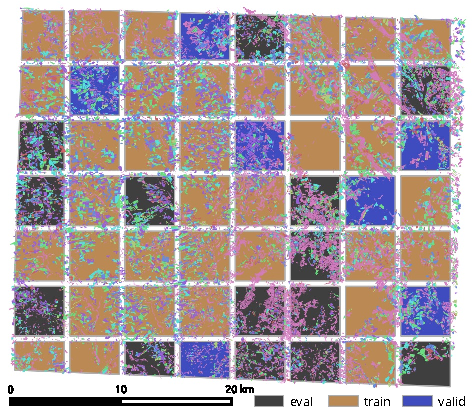
\includegraphics[width=.3\textwidth]{images/holl.pdf}
	\end{minipage}
	\begin{minipage}{.35\textwidth}
%		\tikzsetnextfilename{partition_histograms}
\begin{tikzpicture}
  \centering
  \begin{axis}[
        ybar, axis on top,
        title={},
        height=6cm, width=.8\textwidth,
        bar width=0.3cm,
        ymajorgrids, tick align=inside,
        major grid style={draw=tumgraylight},
        enlarge y limits={value=.1,upper},
        ymin=0, ymax=60,
        axis x line*=bottom,
        axis y line*=left,
        %ymode=log,
        y axis line style={opacity=0},
        tickwidth=0pt,
        enlarge x limits=true,
        legend style={
            at={(1,0.85)},
            anchor=north east,
            draw=none,
            legend columns=-1,
            rounded corners=0,
            /tikz/every even column/.append style={column sep=0.5cm}
        },
        ylabel={\tiny frequency (\%)},
        symbolic x coords={meadows, s. barley,corn,wheat,w. barley,clover,triticale},
       xtick=data,
       ylabel style={yshift=1cm},
       tick label style={rotate=0},
       tick label style={rotate=45,anchor=east},
%       ylabel near ticks,
       %nodes near coords={
       % \tiny \pgfmathprintnumber[precision=0]{\pgfplotspointmeta}
       %}
    ]
    \addplot [draw=none, fill=traincolor] coordinates {
(meadows, 49.506024096385545)
(s. barley, 13.560240963855422)
(corn, 9.632530120481928)
(wheat, 8.072289156626505)
(w. barley, 8.05421686746988)
(clover, 7.530120481927711)
(triticale, 3.644578313253012)
  };
   \addplot [draw=none,fill=validcolor] coordinates {
(meadows, 49.88550866862938)
(s. barley, 13.706247955511941)
(corn, 9.846254497873733)
(wheat, 8.897612037945699)
(w. barley, 8.27608766764802)
(clover, 6.182531894013739)
(triticale, 3.205757278377494)
  };
   \addplot [draw=none, fill=evalcolor] coordinates {
(meadows, 57.32753103801357)
(s. barley, 11.852041469345961)
(corn, 8.524254447715347)
(wheat, 6.962754383719442)
(w. barley, 6.220401894278766)
(clover, 4.876487904774095)
(triticale, 4.236528862152822)
  };

    \legend{train,valid,eval}
  \end{axis}
  \end{tikzpicture}
		\tiny {\color{tumblue}regions with labels} and \\ {\color{tumorange} location of dataset. \par} \par
		\includegraphics[width=.9\textwidth]{images/oberfrankenineurope.pdf}
		 
		 \tiny partition in {\color{traincolor} train}, {\color{validcolor} validation}, and {\color{evalcolor} evaluation} \par
		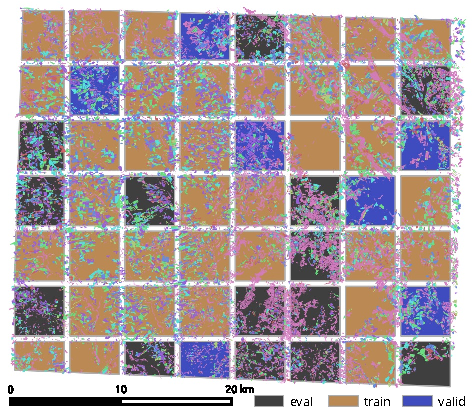
\includegraphics[width=.9\textwidth]{images/holl.pdf}
	\end{minipage}
	
	\end{minipage}

\end{minipage}
\hfill
\begin{minipage}[t]{.32\textwidth}
	\section{Results}
	
	\subsection{Qualitative Example} \par
	{\footnotesize Single example showing reflectance data $\M{x}$ and predictions $\yhat$ along with the stopping time $\tstop \sim \text{Ber}(\deltat)$. \par}
	
	\vspace{.5em}
	\tikzsetnextfilename{example}
\begin{tikzpicture}[rounded corners=0pt]
	
	\tikzstyle{annot} = [font=\verytiny\sffamily, text=tumblue]
	\tikzstyle{point} = [very thin, tumbluelight, shorten >= .25em, shorten <= .25em]
	
	% from /home/marc/projects/EV2019/images/example/tstop.txt
	\def\tstopv{0.6285714285714286}
	\def\class{winter barley}
	
	\begin{groupplot}[
	group style={
		group name=my plots,
		group size=1 by 2,
		columns=1,
		xlabels at=edge bottom,
		xticklabels at=edge bottom,
		vertical sep=1em,
	},
	ylabel near ticks,
	ylabel style={font=\sffamily\small, rotate=-90},
	width=.9\textwidth,
	height=5cm,
	axis x line=bottom,
	axis y line=left,
	enlarge x limits=0.01,
	xtick={0,0.25,0.5,0.75,1},
	xticklabels={January,April,June,Sepember,December},
	ymajorgrids,
	ymin=0, ymax=1.4
	]
	
	\nextgroupplot[very thin,
		no marks,  
		ylabel={$\M{x}$},
		draw opacity=.8,
		smooth,
		legend columns=2,
		legend style={at={(.5,1.2)},anchor=south, line width=1pt, fill=tumblue!10}
		]
		 
	\addplot[b1color] table [x=t, y=B1, col sep=comma, forget plot] {images/example/input.csv};
	\addplot[b9color] table [x=t, y=B9, col sep=comma, forget plot] {images/example/input.csv};
	\addplot[b10color] table [x=t, y=B10, col sep=comma] {images/example/input.csv};
	
	\addplot[b11color] table [x=t, y=B11, col sep=comma, forget plot] {images/example/input.csv};
	\addplot[b12color] table [x=t, y=B12, col sep=comma] {images/example/input.csv};
	
	\addplot[b5color] table [x=t, y=B5, col sep=comma, forget plot] {images/example/input.csv};
	\addplot[b6color] table [x=t, y=B6, col sep=comma, forget plot] {images/example/input.csv};
	\addplot[b7color] table [x=t, y=B7, col sep=comma, forget plot] {images/example/input.csv};
	\addplot[b8color] table [x=t, y=B8, col sep=comma, forget plot] {images/example/input.csv};
	\addplot[b8Acolor] table [x=t, y=B8A, col sep=comma] {images/example/input.csv};
		
	\addplot[b2color] table [x=t, y=B2, col sep=comma, forget plot] {images/example/input.csv};
	\addplot[b3color] table [x=t, y=B3, col sep=comma, forget plot] {images/example/input.csv};
	\addplot[b4color] table [x=t, y=B4, col sep=comma] {images/example/input.csv};
	
	
	\draw[fill=white, draw=none, opacity=.5] (axis cs:\tstopv,0) rectangle (axis cs:1,1.1);
	
	\node[annot](cllab) at (axis cs:.2,1.3) {clouds (noise)};
	\draw[point] (cllab) -- (axis cs:.13,.7);
	\draw[point] (cllab) -- (axis cs:.25,.7);
	\draw[point] (cllab) -- (axis cs:.53,1);
	\draw[point] (cllab) -- (axis cs:.45,.85);
	
	\node[annot](glab) at (axis cs:.9,1.3) {ground (signal)};
	\draw[point] (glab) -- (axis cs:.38,.3);
	\draw[point] (glab) -- (axis cs:.21,.3);
	\draw[point] (glab) -- (axis cs:.7,.3);
	
	\draw (axis cs:\tstopv,0) -- (axis cs:\tstopv,1) node[above, font=\tiny]{$\tstop(\deltat)$};
	
	
	
	\legend{3 atmospheric bands, 2 short-wave infrared bands, 5 near infrared bands, 3 visible bands (RGB)}
	
	
	\nextgroupplot[very thin,
		smooth,
		no marks, 
		ylabel={$\yhat$},
		legend style={at={(.5,-.5)},anchor=north, line width=1pt, fill=tumblue!10, font=\scriptsize},
		legend columns=4]	
	
	\addplot[meadowcolor] table [x=t, y=meadows, col sep=comma] {images/example/proba.csv};
	\addplot[wbarleycolor, thick] table [x=t, y=winter barley, col sep=comma] {images/example/proba.csv};
	\addplot[corncolor] table [x=t, y=corn, col sep=comma] {images/example/proba.csv};
	\addplot[wheatcolor,] table [x=t, y=winter wheat, col sep=comma] {images/example/proba.csv};
	\addplot[sbarleycolor] table [x=t, y=summer barley, col sep=comma] {images/example/proba.csv};
	\addplot[clovercolor] table [x=t, y=clover, col sep=comma] {images/example/proba.csv};
	\addplot[triticalecolor] table [x=t, y=winter triticale, col sep=comma] {images/example/proba.csv};
	
	\draw[fill=white, draw=none, opacity=.5] (axis cs:\tstopv,0) rectangle (axis cs:1,1);
	
	\draw (axis cs:\tstopv,0) -- (axis cs:\tstopv,2.2);
	
	\node[annot](rand) at (axis cs:.1,.8) {first hints};
	\draw[point] (rand) -- (axis cs:.2,.15);
	
	\node[annot](wrong) at (axis cs:.17,1.1) {initially wrong predictions};
	\draw[point] (wrong) -- (axis cs:.25,.7);
	\draw[point] (wrong) -- (axis cs:.4,1);
	
	\node[annot, align=center](corrwait) at (axis cs:.4,1.3) {waiting for more data};
	\draw[point] (corrwait) -- (axis cs:.5,.8);
	
	\node[annot](corr) at (axis cs:.8,1.3) {seen enough data};
	\draw[point] (corr) -- (axis cs:.63,1);
	
	\legend{meadows,\textbf{winter barley},corn,winter wheat,summer barley,clover,winter triticale}
	
	
%	\addplot[thick,colorclassone, name path=y1] table[x=t, y=y1]{\mydata};
%	\addplot[thick,colorclasstwo, name path=y2] table[x=t, y=y2]{\mydata};
%	\addplot[thick,colorclassthree, name path=y3] table[x=t, y=y3]{\mydata};
%	\addplot[thick,colorclassfour, name path=y4] table[x=t, y=y4]{\mydata};
	%\addplot[colorblue!20] fill between[of = y1 and axis];
	%\addplot[colorhgray!20] fill between[of = y2 and axis];
	%\addplot[colorgreen!20] fill between[of = y3 and axis];
	%\addplot[colororange!20] fill between[of = y4 and axis];
	
	
	\end{groupplot}
	
%	\node[font=\sffamily\tiny, anchor=west] at (-.4,3.3) {All 13 spectral bands of the Sentinel 2 satellites grouped by spectral signature};
%	\node[font=\sffamily\tiny, anchor=west] at (0,-3.1) {predicted crop type classes (correct class in \textbf{bold})};
%	
	\end{tikzpicture}
	\vspace{-.5em}
	
	\subsection{Losses during Training} \par
	{\footnotesize The combined loss $L_t$, as well as earliness $L_e$ and accuracy $L_e$ losses during training. \par}

	\vspace{.5em}	
	\newcommand{\figearlyreward}{
\def\datapath{images/logs/data/early_reward_p2/classes}
\tikzsetnextfilename{loss-accuracyplots}
\begin{tikzpicture}
	\begin{groupplot}[
	group style = {
		group size = 1 by 2,
		x descriptions at=edge bottom,
		vertical sep=1em},
	no markers,
	height=5cm,
%	legend style={at={(0.03,0.5)},anchor=west},
	width=\linewidth,
	xlabel=epochs
 	]
	\nextgroupplot[legend columns=3, ylabel=loss]

	\addplot[test, tumblack] table [x=epoch, y=loss, col sep=comma] {\datapath/log_earliness_test.csv};
	
	\addplot[test, accuracycolor] table [x=epoch, y=loss_classification, col sep=comma] {\datapath/log_earliness_test.csv};
	
	\addplot[test, earlinesscolor] table [x=epoch, y=earliness_reward, col sep=comma] {\datapath/log_earliness_test.csv};
	
%	\legend{total loss (eval), classification loss (eval), earliness reward (eval)}
%	
	\legend{$(\mathcal{L}_\text{c} - \mathcal{R}_\text{e})$, $\mathcal{L}_\text{c}$, $\mathcal{R}_\text{e}$}
	
	
	
	\nextgroupplot[
		legend columns=2, 
		legend pos=south east,
		ytick={0,0.5,1},
		yticklabels={
			0 ({\color{earlinesscolor} jan}),
			0.5 ({\color{earlinesscolor} jun}),
			1 ({\color{earlinesscolor} dec})},
		ylabel=accuracy/$\meantstop$]
	\addplot[test, accuracycolor] table [x=epoch, y=accuracy, col sep=comma] {\datapath/log_earliness_test.csv};
	\addplot[test, earlinesscolor] table [x=epoch, y=earliness, col sep=comma] {\datapath/log_earliness_test.csv};

	\legend{accuracy,$\meantstop$}
	
	\end{groupplot}
\end{tikzpicture}

}

\newcommand{\figtwophasecrossentropy}{
\begin{tikzpicture}
\begin{groupplot}[
group style = {
	group size = 1 by 2,
	x descriptions at=edge bottom,
	vertical sep=1em},
no markers,
height=2.8cm,
%	legend style={at={(0.03,0.5)},anchor=west},
width=\linewidth,
ymin=0,ymax=2.5,
xlabel=epochs
]
\nextgroupplot[legend columns=3, ylabel=loss,
legend style={at={(1,.85)}, anchor=north east}]

\addplot[test, tumblack] table [x=epoch, y=loss, col sep=comma] {images/logs/data/twophasecrossentropy/log_earliness_test.csv};

\addplot[test, accuracycolor] table [x=epoch, y=loss_classification, col sep=comma] {images/logs/data/twophasecrossentropy/log_earliness_test.csv};

\addplot[test, earlinesscolor] table [x=epoch, y=loss_earliness, col sep=comma] {images/logs/data/twophasecrossentropy/log_earliness_test.csv};

\draw[draw, thick] (axis cs:50,0) -- (axis cs:50,2) node[above, font=\sffamily\scriptsize](s){switch epoch};
\node[left=1em of s, font=\sffamily\scriptsize]{accuracy only};
\node[right=1em of s, font=\sffamily\scriptsize]{accuracy+earliness};

\legend{$(\mathcal{L}_\text{c} + \mathcal{L}_\text{e})$, $\mathcal{L}_\text{c}$, $\mathcal{L}_\text{e}$}

\nextgroupplot[
legend columns=2, 
ytick={0,0.5,1},
ymin=0,ymax=1,
legend style={at={(1,0)}, anchor=south east},
yticklabels={
	0 ({\color{earlinesscolor} jan}),
	0.5 ({\color{earlinesscolor} jun}),
	1 ({\color{earlinesscolor} dec})},
ylabel=accuracy/$\meantstop$]
\addplot[test, accuracycolor] table [x=epoch, y=accuracy, col sep=comma] {images/logs/data/twophasecrossentropy/log_earliness_test.csv};
\addplot[test, earlinesscolor] table [x=epoch, y=earliness, col sep=comma] {images/logs/data/twophasecrossentropy/log_earliness_test.csv};

\legend{accuracy,$\meantstop$}

\draw[draw, thick] (axis cs:50,0) -- (axis cs:50,1.1);

\end{groupplot}
\end{tikzpicture}

}
	\vspace{-1em}

	\subsection{Stopping Condition Parameterization} \par
	{\footnotesize Stopping times throughout the training grouped by crop category. The parameterization of early classification is learned for different crop types at different times during training. \par}
	
	\def\datapath{images/logs/data/early_reward_p2/classes}

\tikzsetnextfilename{trainingstoppingclasses}
\begin{tikzpicture}
	\begin{groupplot}[
	group style = {
		group size = 1 by 2,
		x descriptions at=edge bottom,
		vertical sep=.75em},
	title style={
		font=\sffamily\scriptsize,
		at={(0,1.1)},
		anchor=north west
	},
	ymajorgrids,
	no markers,
	height=5cm,
	legend style={at={(0.5,1)},anchor=south},
	width=.9\textwidth,
	xlabel=epochs,
	ymax=1.1,
	ymin=0.3,
	ylabel=$\tstop$,
	ylabel style={yshift=1em},
	xlabel style={yshift=-.5em},
	ytick={0,0.25,0.5,0.75,1},
	xtick={0, 10,...,100},
	yticklabels={jan,apr,jun,sep,dec}
	]
	\nextgroupplot[title=meadows, legend columns=3]
	\addplot[meancolor] table [x=epoch, y=meadows, col sep=comma] {\datapath/mean.csv};
	\addplot[mediancolor] table [x=epoch, y=meadows, col sep=comma] {\datapath/median.csv};
	\addplot+[name path=upper, draw=none,forget plot] table [x=epoch, y=meadows, col sep=comma] {\datapath/mean+std.csv};
	\addplot+[name path=lower, draw=none,forget plot] table [x=epoch, y=meadows, col sep=comma] {\datapath/mean-std.csv};
	\addplot[stdcolor] fill between[of=lower and upper];
	
	\legend{mean, median, mean $\mp$ std}
	
	\nextgroupplot[title=winter barley]
	\addplot[meancolor] table [x=epoch, y=winter barley, col sep=comma] {\datapath/mean.csv};
	\addplot[mediancolor] table [x=epoch, y=winter barley, col sep=comma] {\datapath/median.csv};
	\addplot+[name path=upper, draw=none] table [x=epoch, y=winter barley, col sep=comma] {\datapath/mean+std.csv};
	\addplot+[name path=lower, draw=none] table [x=epoch, y=winter barley, col sep=comma] {\datapath/mean-std.csv};
	\addplot[stdcolor] fill between[of=lower and upper];
	
%	\nextgroupplot[title=corn]
%	\addplot[meancolor] table [x=epoch, y=corn, col sep=comma] {\datapath/mean.csv};
%	\addplot[mediancolor] table [x=epoch, y=corn, col sep=comma] {\datapath/median.csv};
%	\addplot+[name path=upper, draw=none] table [x=epoch, y=corn, col sep=comma] {\datapath/mean+std.csv};
%	\addplot+[name path=lower, draw=none] table [x=epoch, y=corn, col sep=comma] {\datapath/mean-std.csv};
%	\addplot[stdcolor] fill between[of=lower and upper];
%	
%	\nextgroupplot[title=winter wheat]
%	\addplot[meancolor] table [x=epoch, y=winter wheat, col sep=comma] {\datapath/mean.csv};
%	\addplot[mediancolor] table [x=epoch, y=winter wheat, col sep=comma] {\datapath/median.csv};
%	\addplot+[name path=upper, draw=none] table [x=epoch, y=winter wheat, col sep=comma] {\datapath/mean+std.csv};
%	\addplot+[name path=lower, draw=none] table [x=epoch, y=winter wheat, col sep=comma] {\datapath/mean-std.csv};
%	\addplot[stdcolor] fill between[of=lower and upper];
%	
%	\nextgroupplot[title=summer barley]
%	\addplot[meancolor] table [x=epoch, y=summer barley, col sep=comma] {\datapath/mean.csv};
%	\addplot[mediancolor] table [x=epoch, y=summer barley, col sep=comma] {\datapath/median.csv};
%	\addplot+[name path=upper, draw=none] table [x=epoch, y=summer barley, col sep=comma] {\datapath/mean+std.csv};
%	\addplot+[name path=lower, draw=none] table [x=epoch, y=summer barley, col sep=comma] {\datapath/mean-std.csv};
%	\addplot[stdcolor] fill between[of=lower and upper];
%	
%	\nextgroupplot[title=clover]
%	\addplot[meancolor] table [x=epoch, y=clover, col sep=comma] {\datapath/mean.csv};
%	\addplot[mediancolor] table [x=epoch, y=clover, col sep=comma] {\datapath/median.csv};
%	\addplot+[name path=upper, draw=none] table [x=epoch, y=clover, col sep=comma] {\datapath/mean+std.csv};
%	\addplot+[name path=lower, draw=none] table [x=epoch, y=clover, col sep=comma] {\datapath/mean-std.csv};
%	\addplot[stdcolor] fill between[of=lower and upper];
%	
%	\nextgroupplot[title=winter triticale]
%	\addplot[meancolor] table [x=epoch, y=winter triticale, col sep=comma] {\datapath/mean.csv};
%	\addplot[mediancolor] table [x=epoch, y=winter triticale, col sep=comma] {\datapath/median.csv};
%	\addplot+[name path=upper, draw=none,forget plot] table [x=epoch, y=winter triticale, col sep=comma] {\datapath/mean+std.csv};
%	\addplot+[name path=lower, draw=none,forget plot] table [x=epoch, y=winter triticale, col sep=comma] {\datapath/mean-std.csv};
%	\addplot[stdcolor] fill between[of=lower and upper];

	
	\end{groupplot}
	\end{tikzpicture}
	
	\subsection{Balancing Earliness and Accuracy} \par
	{\footnotesize Evaluting the effect of the trade-off parameter $\alpha$ on the accuracy and earliness ($\tstop$). Runs repeated three times to evaluated the sability of the results. \par}
	
	\begin{table}
		
		\scriptsize
		\hspace{0em}\begin{tabular}{lcccccc}
			\toprule\small
			\textbf{$\alpha$} & accuracy & $\meantstop$  & precision & recall & $f_1$ & $\kappa$ \\
			\cmidrule(lr){0-0}\cmidrule(lr){1-1}\cmidrule(lr){2-2}\cmidrule(lr){3-3}\cmidrule(lr){4-4}\cmidrule(lr){5-5}\cmidrule(lr){6-6}\cmidrule(lr){7-7}
			.0 & .25 $\pm$ .22 & .10 $\pm$ .17 & .19 $\pm$ .20 & .25 $\pm$ .17 & .16 $\pm$ .20 & .12 $\pm$ .19 \\
			.2 & .81 $\pm$ .03 & .40 $\pm$ .02 & .70 $\pm$ .01 & .74 $\pm$ .01 & .71 $\pm$ .01 & .71 $\pm$ .04 \\
			.4 & .80 $\pm$ .09 & .47 $\pm$ .03 & .71 $\pm$ .02 & .74 $\pm$ .01 & .71 $\pm$ .02 & .71 $\pm$ .10 \\
			.6 & .85 $\pm$ .02 & .88 $\pm$ .07 & .73 $\pm$ .04 & .74 $\pm$ .03 & .73 $\pm$ .03 & .77 $\pm$ .03 \\
			.8 & .84 $\pm$ .01 & .93 $\pm$ .05 & .72 $\pm$ .02 & .75 $\pm$ .01 & .73 $\pm$ .02 & .76 $\pm$ .02 \\
			1.0 & .83 $\pm$ .03 & 1.00 $\pm$ .00 & .72 $\pm$ .03 & .75 $\pm$ .01 & .72 $\pm$ .03 & .75 $\pm$ .04 \\
			\bottomrule
		\end{tabular}
	
	
		%	\caption{Varying the weighting factor $\alpha$ for \emph{early reward} loss formulation (\cref{sec:earlynessreward}).}
		%	\label{tab:alpha}
		
	\end{table}
	
	
	\subsection{Extracting Vegetation Characteristics} \par
	
	{\footnotesize Stopping time per crop category reveals characteristic variations in type of vegetation confirmed by date of harvest (\druschdatum) from local authorities. \par} 
	\vspace{.5em}
	\tikzsetnextfilename{classboxplots}
\begin{tikzpicture}

\tikzstyle{boxstyle}=[
	mark options={
	draw=tumblue,
	scale=0.5},
	mark=*,
	solid,
	draw=black]

\begin{axis}[
ytick={1,2,3,4,5,6,7},
yticklabels={
	meadows,
	winter barley,
	corn,
	winter wheat,
	summer barley,
	clover,
	winter triticale},
xmajorgrids,
xmin = 0,
xmax = 1,
ymin = 1,
ymax = 8,
width=20cm,
height=10cm,
y axis line style={draw=none},
xtick={0,0.1666666667,0.4166666667,0.6666666667,0.9166666667},
xticklabels={January,March,June,September,December},
xlabel={stopping date $\tstop$}
]


%% august <- recommended end of period
% 0.6666666667
\draw [fill=tumbluelight, opacity=.4, draw=none] (axis cs:0.1666666667,0) rectangle (axis cs:0.5833333333,8);
\draw[draw=tumgraydark] (axis cs:0.5833333333,0) -- (axis cs:0.5833333333,8);

\node[font=\tiny\sffamily] at (axis cs:0.37,8.2){vegetative season};

%\node[font=\tiny\sffamily] at (axis cs:0.8,8.2){b};


\addplot+[boxplot, fill=meadowcolor, boxstyle] table[x = meadows, col sep=comma]{images/logs/data/early_reward_p2/classes/meadows.csv};
%
%\addplot+[fill=meadowcolor, draw=black,
%boxplot prepared={
%median=0.4857142857142857,
%upper quartile=0.4,
%lower quartile=0.5857142857142857,
%upper whisker=0.8642857142857143,
%lower whisker=0.12142857142857144,
%} ] coordinates {};

\addplot+[boxplot, fill=wbarleycolor, boxstyle] table[x=winter barley, col sep=comma]{images/logs/data/early_reward_p2/classes/winter_barley.csv};


%
%\addplot+[fill=wbarleycolor, draw=black,
%boxplot prepared={
%median=0.42857142857142855,
%upper quartile=0.37142857142857144,
%lower quartile=0.5857142857142857,
%upper whisker=0.9071428571428573,
%lower whisker=0.04999999999999999,
%} ] coordinates {};


\addplot+[boxplot, fill=corncolor, boxstyle] table[x =corn, col sep=comma]{images/logs/data/early_reward_p2/classes/corn.csv};
%
%\addplot+[fill=corncolor, draw=black,
%boxplot prepared={
%median=0.45714285714285713,
%upper quartile=0.42857142857142855,
%lower quartile=0.5142857142857142,
%upper whisker=0.6428571428571428,
%lower whisker=0.30000000000000004,
%} ] coordinates {};

\addplot+[boxplot, fill=wheatcolor, boxstyle] table[x =winter wheat, col sep=comma]{images/logs/data/early_reward_p2/classes/winter_wheat.csv};


%
%\addplot+[fill=wheatcolor, draw=black,
%boxplot prepared={
%median=0.5285714285714286,
%upper quartile=0.45714285714285713,
%lower quartile=0.5857142857142857,
%upper whisker=0.7785714285714287,
%lower whisker=0.26428571428571423,
%} ] coordinates {};

\addplot+[boxplot, fill=sbarleycolor, boxstyle] table[x =summer barley, col sep=comma]{images/logs/data/early_reward_p2/classes/summer_barley.csv};

%\addplot+[fill=sbarleycolor, draw=black,
%boxplot prepared={
%median=0.37142857142857144,
%upper quartile=0.2857142857142857,
%lower quartile=0.5428571428571428,
%upper whisker=0.9285714285714285,
%lower whisker=-0.09999999999999998,
%} ] coordinates {};

\addplot+[boxplot, fill=clovercolor, boxstyle] table[x=clover, col sep=comma]{images/logs/data/early_reward_p2/classes/clover.csv};

%\addplot+[fill=clovercolor, draw=black,solid,
%boxplot prepared={
%median=0.5,
%upper quartile=0.42857142857142855,
%lower quartile=0.6142857142857143,
%upper whisker=0.892857142857143,
%lower whisker=0.14999999999999986,
%} ] coordinates {};

\addplot+[boxplot, fill=triticalecolor, boxstyle] table[x=winter triticale, col sep=comma]{images/logs/data/early_reward_p2/classes/winter_triticale.csv};

\def\triticale{0.5722222222}
\def\sbarley{0.5833333333}
\def\wbarley{0.5388888889}
\def\wheat{0.5694444444}


% triticale drusch datum 26.07.
%\draw (axis cs:0.524537037,6.5) -- (axis cs:0.524537037,7.5);
\node[druschdatum] at (axis cs:\triticale,7){};

%  summer barley drusch datum 1.8.
%\draw (axis cs:\sbarley,4.5) -- (axis cs:\sbarley,5.5);
\node[druschdatum] at (axis cs:\sbarley,5){};


% winter wheat drusch datum 26.07.
%\draw (axis cs:\wheat,3.5) -- (axis cs:\wheat,4.5);
\node[druschdatum] at (axis cs:\wheat,4){};


% winter barley datum 15.07.
%\draw (axis cs:\wbarley,1.5) -- (axis cs:\wbarley,2.5);
\node[druschdatum] at (axis cs:\wbarley,2){};


%\addplot+[fill=triticalecolor, draw=black,solid,
%boxplot prepared={
%median=0.5571428571428572,
%upper quartile=0.5142857142857142,
%lower quartile=0.6142857142857143,
%upper whisker=0.7642857142857145,
%lower whisker=0.3642857142857141,
%} ] coordinates {};

\end{axis}
\end{tikzpicture} 
	
\end{minipage}

%\frame{
\begin{footer}
	\begin{minipage}{.15\textwidth}
		\textbf{ICML Workshop}\\
		
\includegraphics[width=5cm]{images/AI4SG}
	\end{minipage}
	\begin{minipage}{.275\textwidth}
		\textbf{Technical University of Munich}\footnotemark[1]\\
		TUM Department of Civil, Geo and Env. \\
		Remote Sensing Technology \\
		Arcisstr. 21, 80333 Munich, Germany
	\end{minipage}
	\begin{minipage}{.275\textwidth}
		\textbf{IRISA-Obelix}\footnotemark[2]\\
		Université Bretagne Sud \\
		IRISA, UMR 6074 CNRS \\
		Campus de Tohannic, 56000 Vannes, France
		
	\end{minipage}
	\begin{minipage}{.2\textwidth}
		\textbf{Data \& Code} \\
		%		\vspace{1em}
		{github.com/rtavenar/early\_rnn} \\
		{twitter.com/MarcCoru} \\
		www.lmf.bgu.tum.de/vision
	\end{minipage}
	\begin{minipage}{.05\textwidth}
		\hfill
\includegraphics[width=5cm]{images/qr-code}\\
		
	\end{minipage}

	
\end{footer}
%}

\end{document}